\documentclass{article}
\usepackage{amsmath}
\usepackage{amssymb}
\usepackage{graphicx}

\usepackage[top=1in, bottom=1.25in, left=1.25in, right=1.25in]{geometry}

\newcommand{\mtwotwo}[4]{\begin{bmatrix} #1 & #3 \\ #2 & #4 \end{bmatrix}}
\newcommand{\br}[1]{\left\{#1\right\}}
\newcommand{\brkt}[1]{\left[#1\right]}
\newcommand{\prn}[1]{\left(#1\right)}
\newcommand{\reals}{\mathbb{R}}
\newcommand{\cyc}[1]{\mathbb{Z}_{#1}}
\newcommand{\ints}{\mathbb{Z}}
\newcommand{\rationals}{\mathbb{Q}}
\newcommand{\lcm}{\text{lcm}}
\newcommand{\galois}[1]{\mathbb{F}_{#1}}

\begin{document}
\title{COSC363 -- Assignment 1 -- OpenGL Museum}
\author{Lucas Payne --- 73231707}
\date{}
\maketitle
\vskip -0.2in
\hrule
\vskip 0.03in
\hrule
\vskip 0.2in

\newcommand{\thing}[3]{
\vskip 0.2in
\hrule
\vskip 0.03in
\hrule
\vskip 0.1in
    \textbf{\textit{#3 #1}}:
#2
\vskip 0.1in
\hrule
\vskip 0.03in
\hrule
\vskip 0.2in
}
\newcommand{\exhibit}[2]{\thing{#1}{#2}{Exhibit}}
\newcommand{\feature}[2]{\thing{#1}{#2}{Feature}}
\newcommand{\leadin}[2]{
    \textit{#1}
    \vskip 0.1in
    \hrule
    \vskip 0.08in
    #2
    \vskip 0.6cm
}

I have created the ``Museum of Geometry'', an open-air museum which houses some interesting geometric objects and algorithms.
\begin{center}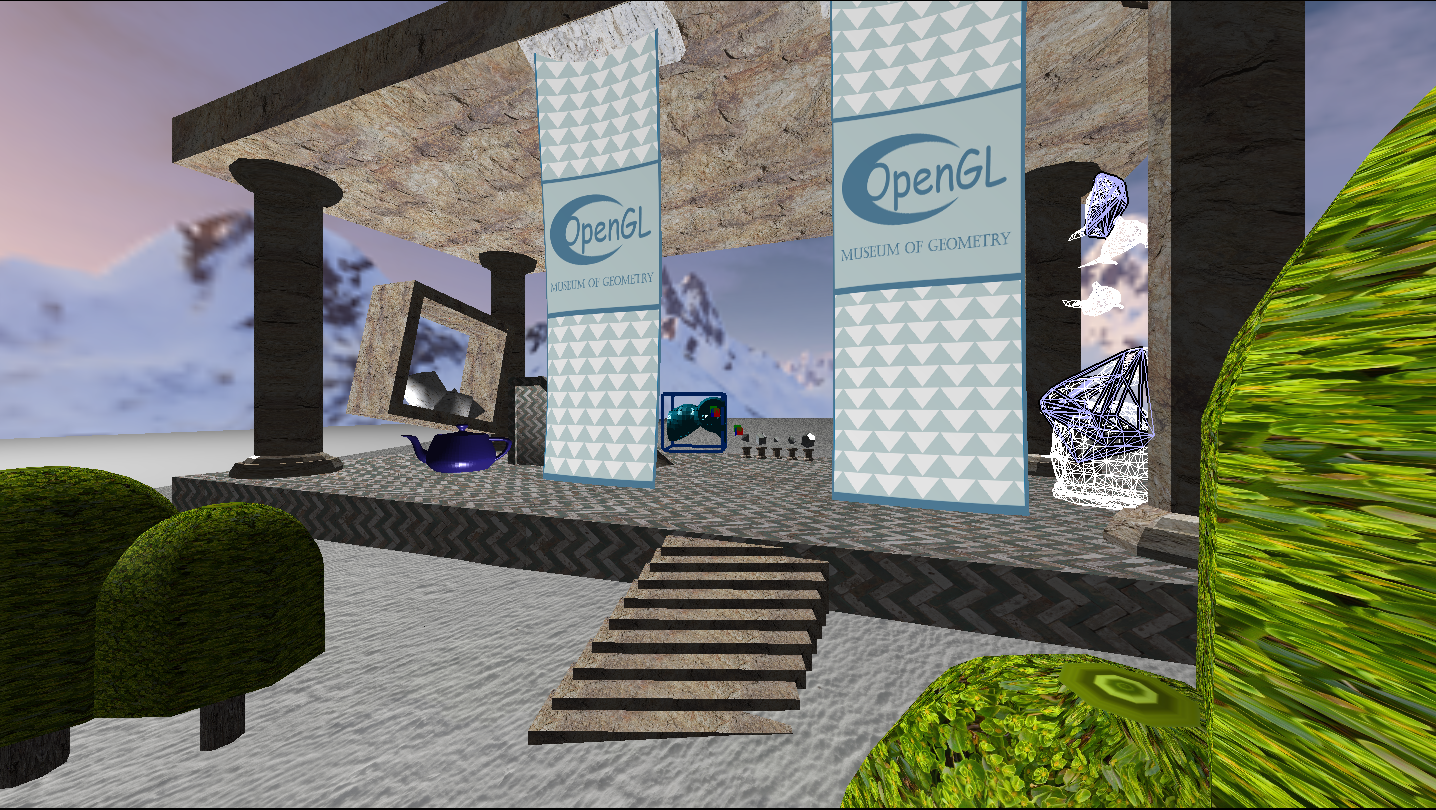
\includegraphics[width=\linewidth]{screenshots/museum_from_outside.png}\end{center}

\leadin{Controls and interaction}{
    The player is controlled using two sets of arrow keys. H,J,K,L are synonymous with Left, Down, Up, Right, respectively.
    W and S or Up and Down move forwards and backwards, while Left and Right turn the player. A and D allow movement
    sideways. There is some mouse interaction with clicking and dragging, using the left mouse button.
    Collision detection is active, and most objects are solid. ESC quits the program. If anything goes wrong, and the player gets
    lost, or there is a collision error, R will reset the player position. 
    {(\scriptsize note: Holding the shift key seems to mess with glut's input functions. If this happens, the program must be reset.)}
}
\leadin{The museum and its exhibits}{
    The museum is open-air, and stands in an icy plain. The sky is a textured box, the base floor is a large solid block, and
    the hills are generated semi-randomly by creating the models as convex hulls of random point clouds. Trees are created as by two surfaces of revolution each.
    The banners are biquartic B\'ezier surfaces, with control points modulated over time to look like they are moving in the wind.

\newpage


\noindent\fbox{%
    \parbox{\textwidth}{%
    \textbf{An overview of the exhibits.}
    \vskip 0.25cm
    \hrule
    \vskip 0.25cm
    \textit{Rigid-body dynamics and collision detection:} A rotating tumbler houses the Platonic solids, showcasing a basic rigid-body physics simulation. Click and drag a Platonic solid to give it some momentum.
        To facilitate physics simulation, collision detection is active, which is also used to make the museum solid and navigable by the player.
    \vskip 0.15cm

    \hrule
    \vskip 0.25cm
    \textit{3D convex hulls:} The iterative algorithm for 3D convex hulls is visualized by building up the convex hulls of the Stanford bunny and a few dolphins, then encasing them in stone.
    \vskip 0.15cm
    
    \hrule
    \vskip 0.25cm
    \textit{Surfaces:} Various displays showcase surface methods. A B\'ezier patch and B\'ezier triangle have control points controllable by widgets, each draggable by mouse across any of the axis planes.
        The Utah teapot has multiple levels of tessellation visualized, alternating from one to four-hundred quads per patch. Metaballs, a certain kind of isosurface, move around in a tank creating an amorphous object.
        These are also draggable with control widgets.
    \vskip 0.15cm

    \hrule
    \vskip 0.25cm
    \textit{Interactive solids:} The Platonic solids are displayed on pillars. Each has a virtual trackball, which can be used rotate it or give it angular momentum.
    \vskip 0.15cm
    \hrule
    }%
}
}
\leadin{Program structure and sources}{
    I have implemented this program with a simplified entity system. Most behaviour is separated from the direct master loop,
    and objects are created as entities. To render them a ModelRenderer is attached, to be collidable a Collider is attached, and so on. All source code is written in C, and
    has been developed using GCC and make on a computer running Linux Mint.

    I have used textures from \textit{https://www.textures.com}, skybox textures from the course web-page, as well as the original B\'ezier patch description of the Utah teapot,
    a low-resolution of the Stanford bunny from Stanford's models repository, and a model of three dolphins acquired from \textit{https://people.sc.fsu.edu/~jburkardt/data/ply/ply.html}.
    All other models have been generated in code by my own procedures, and the banners were created in GIMP.
}

\feature{}{Collision detection.}
    Colliders can be attached to entities, giving them solidity. This allows them to interact with the player, and, for example, to be used in a physics simulation. My main reference
    for this topic has been [Ericson, Real-Time Collision Detection].
    
    The Gilbert-Johnson-Keerthi algorithm, or GJK, is a geometric algorithm for determining contact and distance information between convex objects. I have implemented
    this algorithm for convex polyhedra, along with the expanding polytope algorithm, or EPA, which computes the minimal separating vector.    
    The polyhedra are given as point clouds, which define their convex hulls.
    The GJK algorithm descends a simplex through the Minkowski difference, or configuration space obstacle, of the polyhedra.
    If the simplex ever bounds the origin, the polyhedra are intersecting (as for some
    points $a$ in $A$ and $b$ in $B$, $a - b = 0 \Rightarrow a = b$). This process uses the support function of the CSO, which is conveniently computable
    as a linear combination of support functions of each polyhedron, giving $O(n + m)$ rather than $O(nm)$ time-complexity.
    If they are not intersecting, the closest points of the two polyhedra can be computed from
    the closest point on the CSO to the origin.

    If they are colliding, contact information is wanted. The minimum separating vector is given,
    computed by the expanding polytope algorithm (EPA). This algorithm progressively expands
    a sub-polytope of the CSO in order to find the closest point on the CSO boundary to the origin,
    whose negative is the separating vector, the minimal translation to move the CSO so that it does not
    bound the origin. This can be used to infer the contact normal and contact points on each polyhedron.*

    The implementation works for a demo, but is incomplete, and I will continue making a more robust and efficient system.

    \vskip 0.1in
    {*\scriptsize Denote the closest point to the origin on the CSO $p$. $p$ is on at least one of the triangles of the CSO, and is therefore a convex
    combination of its points, $p = w_1a + w_2b + w_3c,\ 0 \leq w_i \leq 1, w_1 + w_2 + w_3 = 1$. Since each point on the triangle is the difference
    between a point on A and a point on B, $a = a_1 - a_2$, $b = b_1 - b_2$, and $c = c_1 - c_2$, the corresponding points on $A$ and $B$ are then
    $p_1 = w_1a_1 + w_2a_1 + w_3a_1$ and $p_2 = w_1a_2 + w_2a_2 + w_3a_2$. These are considered as the ``points of contact'' on $A$ and $B$.}
    \vskip 0.1in

\feature{}{Virtual trackballs}
A mini-exhibit showcases the Platonic solids on pillars modelled as surfaces of revolution. These solids can be rotated and spun by
clicking and dragging with the mouse. This is done by casting a ray from the camera and intersecting it with a sphere, taking
the change of the point on the sphere being dragged, and constructing an axis-angle matrix to transform the object orientation.
If the mouse is released while dragging, the object will gain some momentum. This is done by giving the object an angular velocity $\omega$,
which updates the object orientation of the object each frame by the equation $R^+ = \left( R^- + \omega^* R^-\Delta t\right)_o$, where $R^{\pm}$ are is the
before/after entity orientation matrix, $\omega^*$ is the skew-symmetric matrix such that $\omega^* u = \omega \times u$, and $(\cdot)_o$ denotes Gram-Schmidt orthonormalization.


\exhibit{A}{3D convex hull algorithm visualization.}
\begin{center}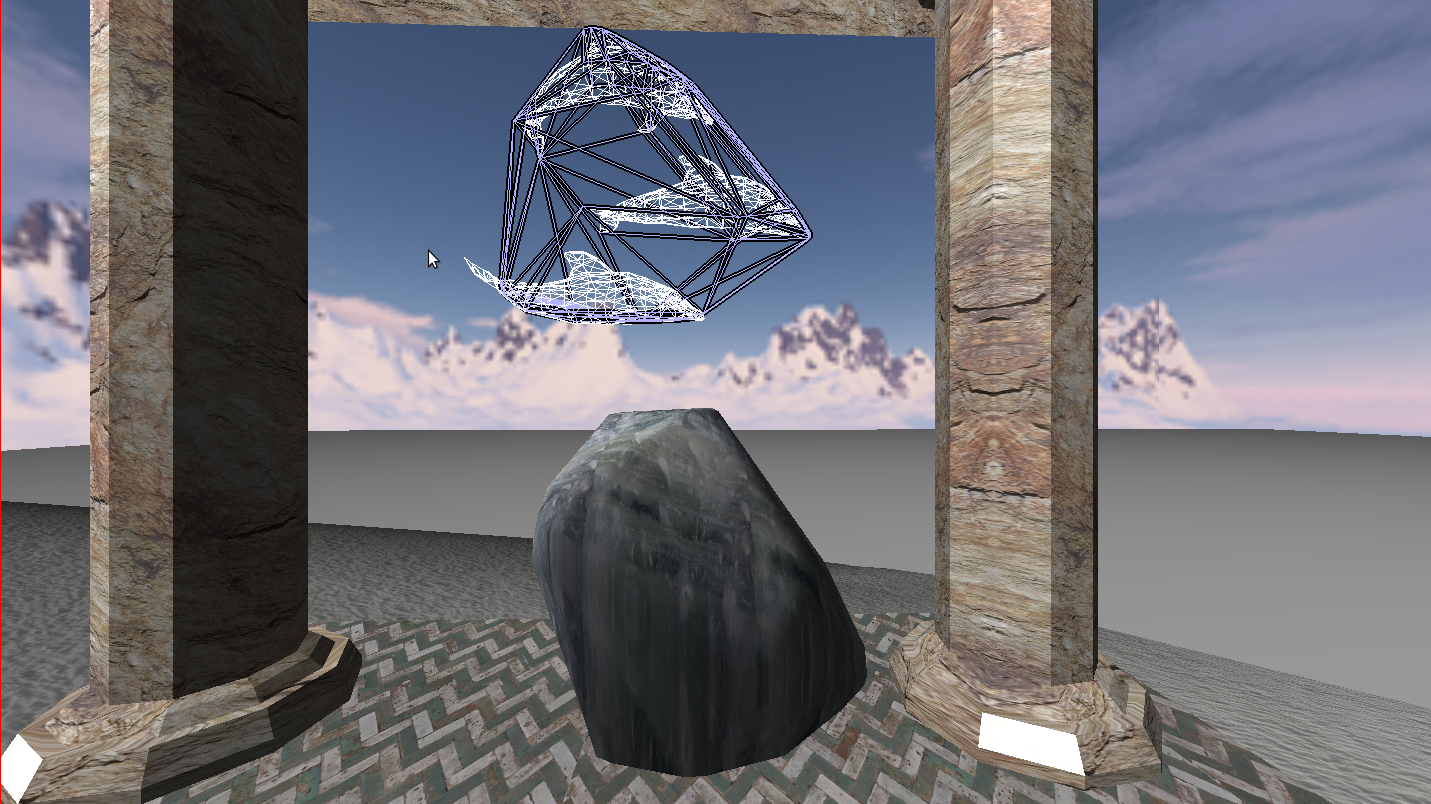
\includegraphics[width=\linewidth]{screenshots/convex_hulls.png}\end{center}
The convex hull of a set of 3D points is a useful geometric object, and is used in other exhibits of the museum. I have implemented an algorithm
for computing the convex hull as a vertex-edge-face polyhedron data structure. The method used is the one described in [O'Rourke, Computational Geometry in C],
called by him the iterative method. This is an $O(n^2)$ method which initializes the convex hull as a tetrahedron consisting of points in the set.
The algorithm iterates over all points, and if the point is outside of the convex hull so far, the hull is extended by finding the boundary of the hull from
the point of view of the new point, deleting the visible faces and other unnecessary features, and adding a cone whose apex is the new point and base is the computed boundary.
The visualization animates the convex hull being built, which when completed, turns to stone.

\exhibit{B}{Rigid body dynamics.}
\begin{center}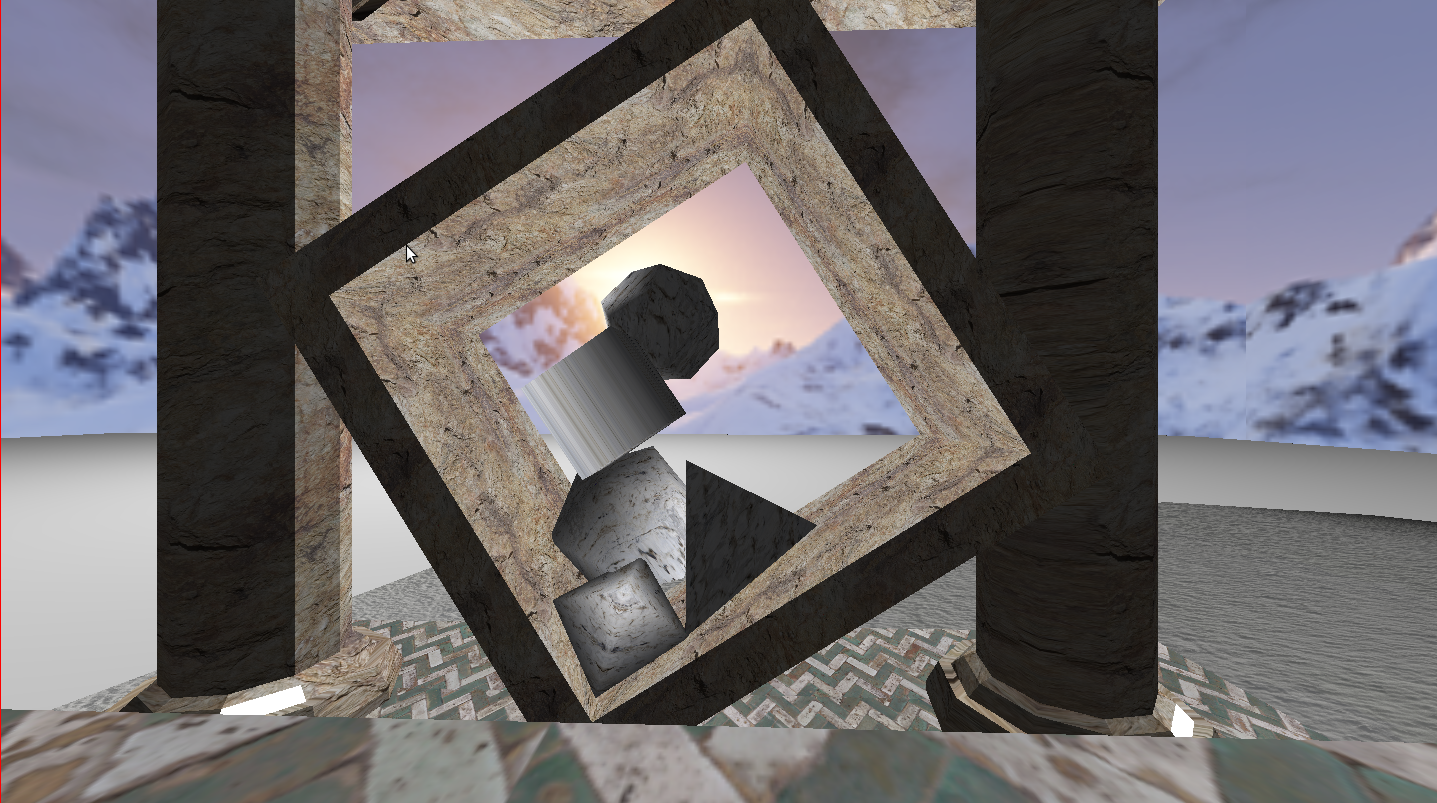
\includegraphics[width=\linewidth]{screenshots/rigid_bodies.png}\end{center}

To the left of the entrance to the museum, the second exhibit showcases the Platonic solids tumbling inside of a rotating frame. This is best viewable on top of the viewing platform.
The Platonic solids can be clicked and dragged around, giving them momentum in the direction the mouse moves.

To do this, collision detection is used as a basis for a basic rigid-body dynamics loop based on impulses. My main references are [Parent, Computer Animation] and [Eberly, Game Physics].
It is wanted for colliders not to interpenetrate. As a simple (non-robust) approximation, each collider can iteratively be pushed along the separating vector of any collision they are in.

The changing state of a rigid body contains the position ($p$) and orientation ($R$), linear momentum ($P$) and angular momentum ($L$). The state kept constant is the mass ($m$)
and the body-space inertia tensor ($J$). The inertia tensor is derived as the linear relationship (as a matrix) between angular momentum and velocity.*
Once these quantities are computed, they are stored in the rigid-body, and a loop integrates rigid-body states, and checks collisions.
\vskip 0.1in
{*\scriptsize
Straight from their definition,
$$L = \int_R \delta r \times v\, dr$$
where $R$ is the region of the body, $\delta$ is the mass density function, and $v$ is the linear velocity at the point with relative position $r$ from the center of mass.
$$v = \omega \times r = -r \times \omega,$$
giving
\begin{align*}
    L &= -\int_R \delta r \times (r \times \omega)\, dr
      = -\int_R \delta (r^*)^2 \omega\, dr
      = \left(-\int_R \delta (r^*)^2\, dr\right) \omega.
\end{align*}
The final term acting on $\omega$ is the inertia tensor, and can be calculated numerically.}

\exhibit{C}{Surfaces.}
\begin{center}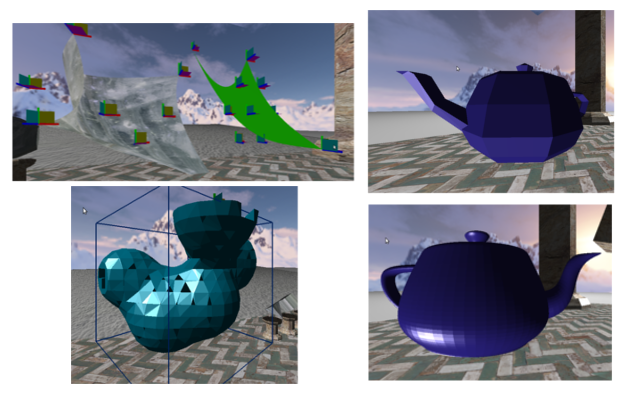
\includegraphics[width=\linewidth]{screenshots/surfaces.png}\end{center}

\vskip 0.1cm
\textit{B\'ezier patch and triangle}
\vskip 0.1cm
\hrule
\vskip 0.2cm
A few surface-rendering and design methods are showcased. The first two are
the rectangular and triangular B\'ezier patches, with control points controllable with the mouse, by
dragging the control widgets via their handles across each axis plane. These surfaces are a generalization
of B\'ezier curves, which are defined via repeated linear interpolation. This repeated interpolation expands to
a basis of polynomials called the Bernstein polynomials, which are used to evaluate the patch at points in its domain:
$0 \leq u,v \leq 1$ for the rectangular patch, and $0 \leq u,v,w \leq 1,\ u + v + w = 1$ for the triangular patch.
These patches are tessellated much like in OpenGL 4, by generating points in the domain connected by a triangle pattern,
which are then mapped to their points in space computed from the points in the patch along with the tessellation coordinates.

\vskip 0.1cm
\textit{The Utah teapot}
\vskip 0.1cm
\hrule
\vskip 0.2cm
The Utah teapot is tessellated as an example of an object made from composite B\'ezier patches, at varying tessellation levels. B\'ezier patches
are also used to model the banners at the entrance to the museum.

\vskip 0.1cm
\textit{Metaballs (isosurfaces)}
\vskip 0.1cm
\hrule
\vskip 0.2cm
Lastly, a quite different surface design method called ``metaballs'' is displayed. While B\'ezier surfaces are parametric,
and thus easily rendered, there are some problems in rendering isosurfaces, level-sets $f(x) = \lambda$ of functions over $\reals^3$. The isosurface
must be found rather than just evaluated.

The approach of ``marching cubes'' is used here, which samples the function $f$
at a grid of points. For each cell of this grid, the predicate $f(c) \leq \lambda$ for each corner $c$
of the cell gives an 8-bit-pattern. By the mean value theorem, if $f$ is continuous, then if this bit pattern is not all zeros or all ones,
the level-set must pass through this cell. A table of triangles to generate for each pattern is used, such that each generated surface element
joins nicely with each adjacent cell. I have generated my own table of cell configurations using a separate program I have written. These seem to be largely correct, but
with some artifacts.

\vskip 0.2in
\hrule
\vskip 0.2in
I really enjoyed this assignment. Curves and surface methods are very interesting. Further additions I would like to program are subdivision surfaces, B-splines, and NURBs patches. I would also like to make a more
robust collision detection system, and a skinned animation system with OpenGL 4.

\end{document}

